\chapter{Resultados}

O problema proposto, o qual os testes serão realizados, se dá no próprio
ambiente de simulação de carros autônomos criado previamente. Neste, serão
aplicados dois diferentes algoritmos de inteligência artificial:

\begin{enumerate}
	\item NEAT, proveniente do \textit{neat-python} pós parametrização; 
	\item Neuroevolução, através da aplicação de um algoritmo genético sobre uma rede neural simples (sem topologias aumentantes);
\end{enumerate}

Tais algoritmos trabalham de diferentes formas a encontrar valores de aptidão
para suas simulações. De modo a generalizar a classificação de resultados, foi
proposto a construção de um valor de pontua{\c c}{\~a}o atrelado à distância percorrida pelo
carro em sua execução.

Esta métrica pode vir a ser comparada entre métodos a fim de se encontrar
quanto tempo é necessário para se alcançar determinada fitness e quanto é
alcançado após determinado tempo de execução decorrer.

Os resultados foram obtidos de duas diferentes formas: primeiramente
encontrando em que geração do algoritmo este consegue alcançar um valor de
\textit{fitness} mínimo necessário para que o carro execute uma volta completa pelo
trajeto, definindo assim quão rapidamente ele consegue alcançar uma resposta. A
\autoref{fig_meta} ilustra dentro do ambiente de simulação o alvo a ser alcançado.

\begin{figure}[htb]
        \centering
        \caption{\label{fig_meta}Canto inferior esquerdo definido como meta a ser alcançada para obtenção de resultado.}
        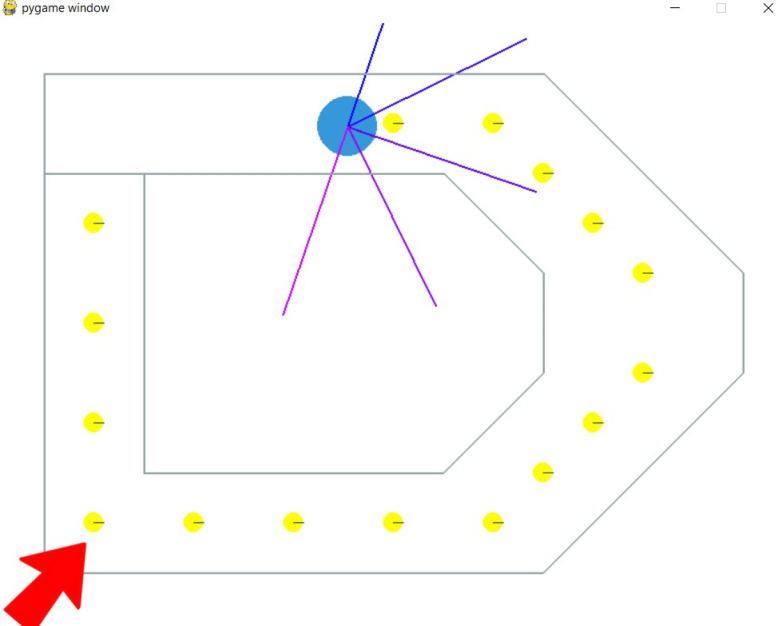
\includegraphics[width=0.5\textwidth]{images/meta.png}
        \legend{
                Fonte: Autoria Pr{\'o}pria.
        }
\end{figure}

A Rede Neural inicial é composta por 5 sensores que verificam e alimentam a
rede a cada movimento do carro e são elencados com os valores que vão de -5 até
-1. Essas 5 entradas estão todas conectadas a cada um das 3 saídas que indicam
a direção que o carro deve tomar, as saídas vão de 0 até 2, sendo 0 a indicação
de movimento a esquerda, 1 a direito e 2 para frente. Cada conexão entre cada
sensor de entrada e cada nó de saída possui um peso específico que serve para a
geração do valor de saída. A estrutura indicada acima pode ser encontrada na
\autoref{fig_nn1} abaixo.

\begin{figure}[htb]
        \centering
        \caption{\label{fig_nn1}Organização da rede, com seus nós e conexões.}
        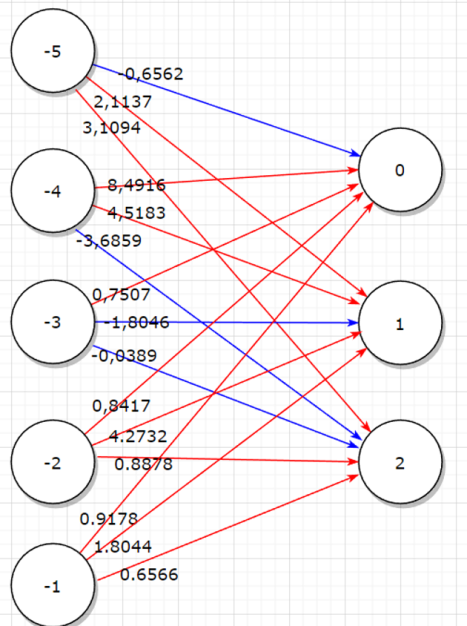
\includegraphics[width=0.4\textwidth]{images/nn1.png}
        \legend{
                Fonte: Autoria Pr{\'o}pria.
        }
\end{figure}

O processo de aprendizado de uma determinada rede veio a ser executado em um
ambiente de treinos, o qual, tratando-se do algoritmo NEAT, a topologia parte
de seu estado mais simples até possuir um determinado formato da qual é capaz
de finalizar o percurso, sendo tratada como a resposta ideal proposta. O
algoritmo de Neuroevolução e também partem de seu estado mais
simples até as respostas desejadas neste ambiente.

\section{NEAT}

A simulação do treino para o algoritmo NEAT incorpora o aumento das topologias,
este pode vir a ser dado pela possibilidade de adições e subtrações de nós nas
camadas ocultas da rede e/ou remoção ou adição de conexões entre nós, fatores
observados nas redes dos resultados alcançados.

Foram realizadas três execuções com o objetivo de se alcançar a fitness mínima
para que uma volta completa seja realizada em torno da pista, mensurado como
cerca de 16000 pontos de aptidão com 300 membros na população. Os resultados
com as respectivas gerações em que o cálculo foi alcançado se dão na \autoref{tabela_neat},
juntamente da topologia resultante em cada iteração.

\begin{table}[htb]
	\centering
    \caption{\label{tabela_neat}Resultados obtidos pelo NEAT até a meta de Fitness ser alcançada.}
    \begin{tabular}{ccccc}
        \hline
		\textbf{Itera{\c c}{\~o}es} & \textbf{Topologia} & \textbf{Gera{\c c}{\~a}o} & \textbf{\textit{Fitness}} & \textbf{\textit{Fitness} média} \\ \hline
		1 & (3,13)  & 8   & 16379  & 3664 ± 2106   \\ \hline
		2 & (3,14)  & 3   & 16337  & 3285 ± 2165   \\ \hline
		3 & (4,13)  & 8   & 16336  & 3684 ± 2126   \\ \hline
    \end{tabular}
    \fonte{Autoria pr{\'o}pria.}
\end{table}

Como observável na \autoref{fig_nn2}, a terceira iteração obteve uma  topologia
a qual indica a existência de quatro nós e treze conexões totais, este nó
intermediário, inserido após um processo de mutação, serve como uma conexão na
camada oculta entre a entrada -2 e as saídas 1 e 2. Além desta alteração, a
topologia também sofreu alterações com a remoção da conexão entre a entrada -3
e saída 0, julgada pelo algoritmo como uma melhoria para o desempenho durante
suas mutações e cruzamentos.

\begin{figure}[htb]
        \centering
        \caption{\label{fig_nn2}Rede neural da Iteração 3 de treinos do algoritmo NEAT, com uma conexão excluída e um nó adicional na camada oculta.}
        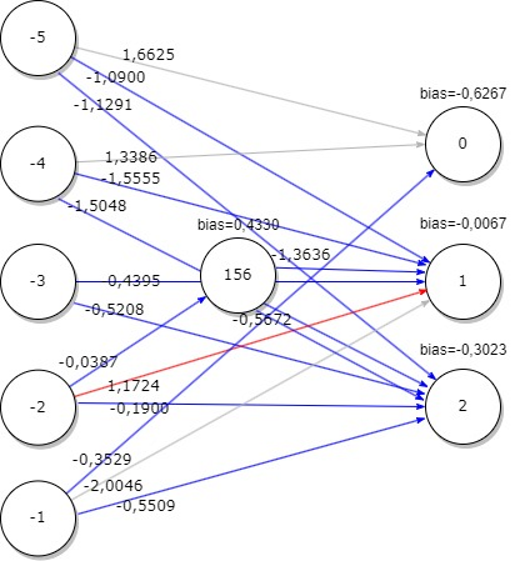
\includegraphics[width=0.4\textwidth]{images/nn2.png}
        \legend{
                Fonte: Autoria Pr{\'o}pria.
        }
\end{figure}

A segunda bateria de treinos englobava a execução do algoritmo até sua 10ª
geração, e a comparação dos resultados obtidos até então. Seus resultados são
observáveis na \autoref{tabela_neat_10}.

\begin{table}[htb]
	\centering
    \caption{\label{tabela_neat_10}Resultados obtidos pelo NEAT após a execução de 10 gerações.}
    \begin{tabular}{ccccc}
        \hline
		\textbf{Itera{\c c}{\~o}es} & \textbf{Topologia} & \textbf{Gera{\c c}{\~a}o} & \textbf{\textit{Fitness}} & \textbf{\textit{Fitness} média} \\ \hline
		1 & (4,9)   & 10  & 16383  & 3191 ± 2524   \\ \hline
		2 & (3,12)  & 10  & 18528  & 3847 ± 1997   \\ \hline
		3 & (4,15)  & 10  & 14199  & 3569 ± 1903   \\ \hline
    \end{tabular}
    \fonte{Autoria pr{\'o}pria.}
\end{table}

Observando a topologia da iteração de número 2, é possível verificar que esta
que obteve o melhor resultado com o mesmo tempo de execução das demais,
identificou como uma melhora no resultado a quebra da conexão entre a entrada
-5 e a saída 0 e a entrada -1 e saída 2, como observável na \autoref{fig_nn3}.

\begin{figure}[htb]
        \centering
        \caption{\label{fig_nn3}Rede neural da Iteração 2 de treinos do algoritmo NEAT, com duas conexões excluídas e uma desativada.}
        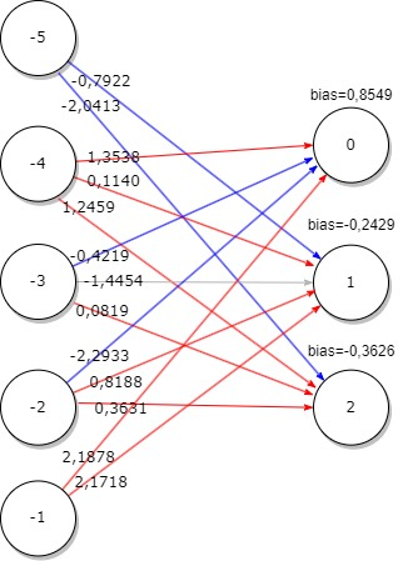
\includegraphics[width=0.4\textwidth]{images/nn3.png}
        \legend{
                Fonte: Autoria Pr{\'o}pria.
        }
\end{figure}

\section{Neuroevolu{\c c}{\~a}o}

Para a simulação de um algoritmo básico de Neuroevolução sem a etapa de aumento
de topologias, se fez uso da mesma estrutura utilizada anteriormente pelo NEAT,
porém sem a possibilidade de haver adições ou subtrações de nós (nas camadas
ocultas) ou conexões (entre entradas, nós e saídas).

Como apresentado na \autoref{tabela_ne}, o algoritmo foi executado três vezes com
diferentes valores para \textit{fitness} alcançada e em que geração esta se deu,
considerando uma população de 300 integrantes.

A coluna de formato da rede não se faz necessária considerando que este, por se
tratar de um algoritmo simples de neuroevolução, possui suas tomadas de
decisões realizadas apenas na pesagem de suas arestas, sem alterações de
topologia durante a execução.

\begin{table}[htb]
	\centering
    \caption{\label{tabela_ne}Resultados obtidos em suas respectivas gerações após execução do algoritmo de Neuroevolução.}
    \begin{tabular}{cccc}
        \hline
		\textbf{Itera{\c c}{\~o}es} & \textbf{Gera{\c c}{\~a}o} & \textbf{\textit{Fitness}} & \textbf{\textit{Fitness} média} \\ \hline
		1 & 3   & 16345  & 3354 ± 2138   \\ \hline
		2 & 12  & 16373  & 3839 ± 1930   \\ \hline
		3 & 12  & 16382  & 3788 ± 2298   \\ \hline
    \end{tabular}
    \fonte{Autoria pr{\'o}pria.}
\end{table}

A rede neural referente à iteração que alcançou o resultado mais rapidamente
pode ser expressa na \autoref{fig_nn4}, com suas devidas conexões e pesos.

\begin{figure}[htb]
        \centering
        \caption{\label{fig_nn4}Rede neural da Iteração 1 de treinos do algoritmo de Neuroevolução.}
        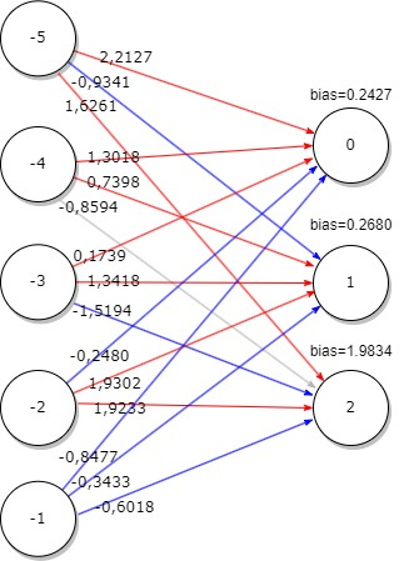
\includegraphics[width=0.4\textwidth]{images/nn4.png}
        \legend{
                Fonte: Autoria Pr{\'o}pria.
        }
\end{figure}

A \autoref{tabela_ne_10} ilustra os resultados obtidos para o algoritmo de
Neuroevolução considerando três execuções até a décima geração, com a fitness
média e máxima alcançadas dentro da população de 300 integrantes para cada
iteração. Do mesmo modo, a rede neural com o resultado da iteração de melhor
resultado pode ser expressa na \autoref{fig_nn5}, com suas devidas conexões e
pesos.

\begin{table}[htb]
	\centering
    \caption{\label{tabela_ne_10}Resultados obtidos até a décima geração após execução do algoritmo de Neuroevolução.}
    \begin{tabular}{cccc}
        \hline
		\textbf{Itera{\c c}{\~o}es} & \textbf{Gera{\c c}{\~a}o} & \textbf{\textit{Fitness}} & \textbf{\textit{Fitness} média} \\ \hline
		1 & 10  & 16356  & 3754 ± 2159   \\ \hline
		2 & 10  & 19596  & 3923 ± 2101   \\ \hline
		3 & 10  & 16335  & 3767 ± 1966   \\ \hline
    \end{tabular}
    \fonte{Autoria pr{\'o}pria.}
\end{table}

\begin{figure}[htb]
        \centering
        \caption{\label{fig_nn5}Rede neural da Iteração 2 após 10 gerações de treinos do algoritmo de Neuroevolução.}
        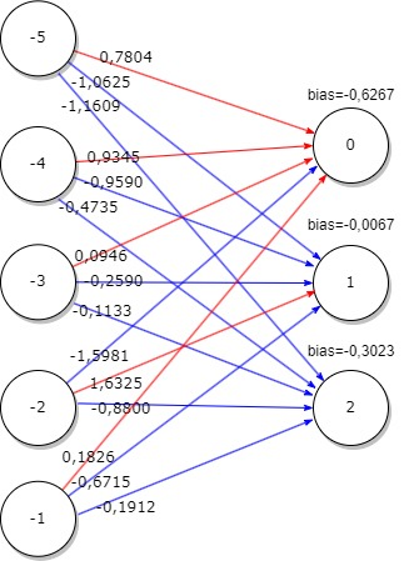
\includegraphics[width=0.4\textwidth]{images/nn5.png}
        \legend{
                Fonte: Autoria Pr{\'o}pria.
        }
\end{figure}
